We conducted two different experiments, one to predict the force measured
by the force sensor and another one to classify the grasp type.
%The EMG data were preprocessed as described in Section \ref{sec:preproc}.

As already mentioned in Section \ref{sec:adapt}, our working
assumption is to have $N$ pre-trained models stored in memory; new
data comes from subject $N+1$ and the system starts training, to build
the $N+1$'th model. The performance is then evaluated using unseen
data from subject $N+1$. To simulate this scenario and to have a
reliable estimation of the performance, we use a leave-one-out
approach: out of the $10$ subjects for which we have data recordings,
we train $9$ models off-line. These correspond to the $N$ stored
models in memory, while data from the remaining subject are  used
for the adaptive learning of the $N+1$'th model. The training
sequences are random subsets from the entire dataset, that is they are taken
without considering the order in which they were acquired. This
procedure is repeated $10$ times, using in turn all the recorded
subjects for the adaptive learning of the model.

\begin{figure*}[!ht] \centering
  \begin{tabular}{cc}
    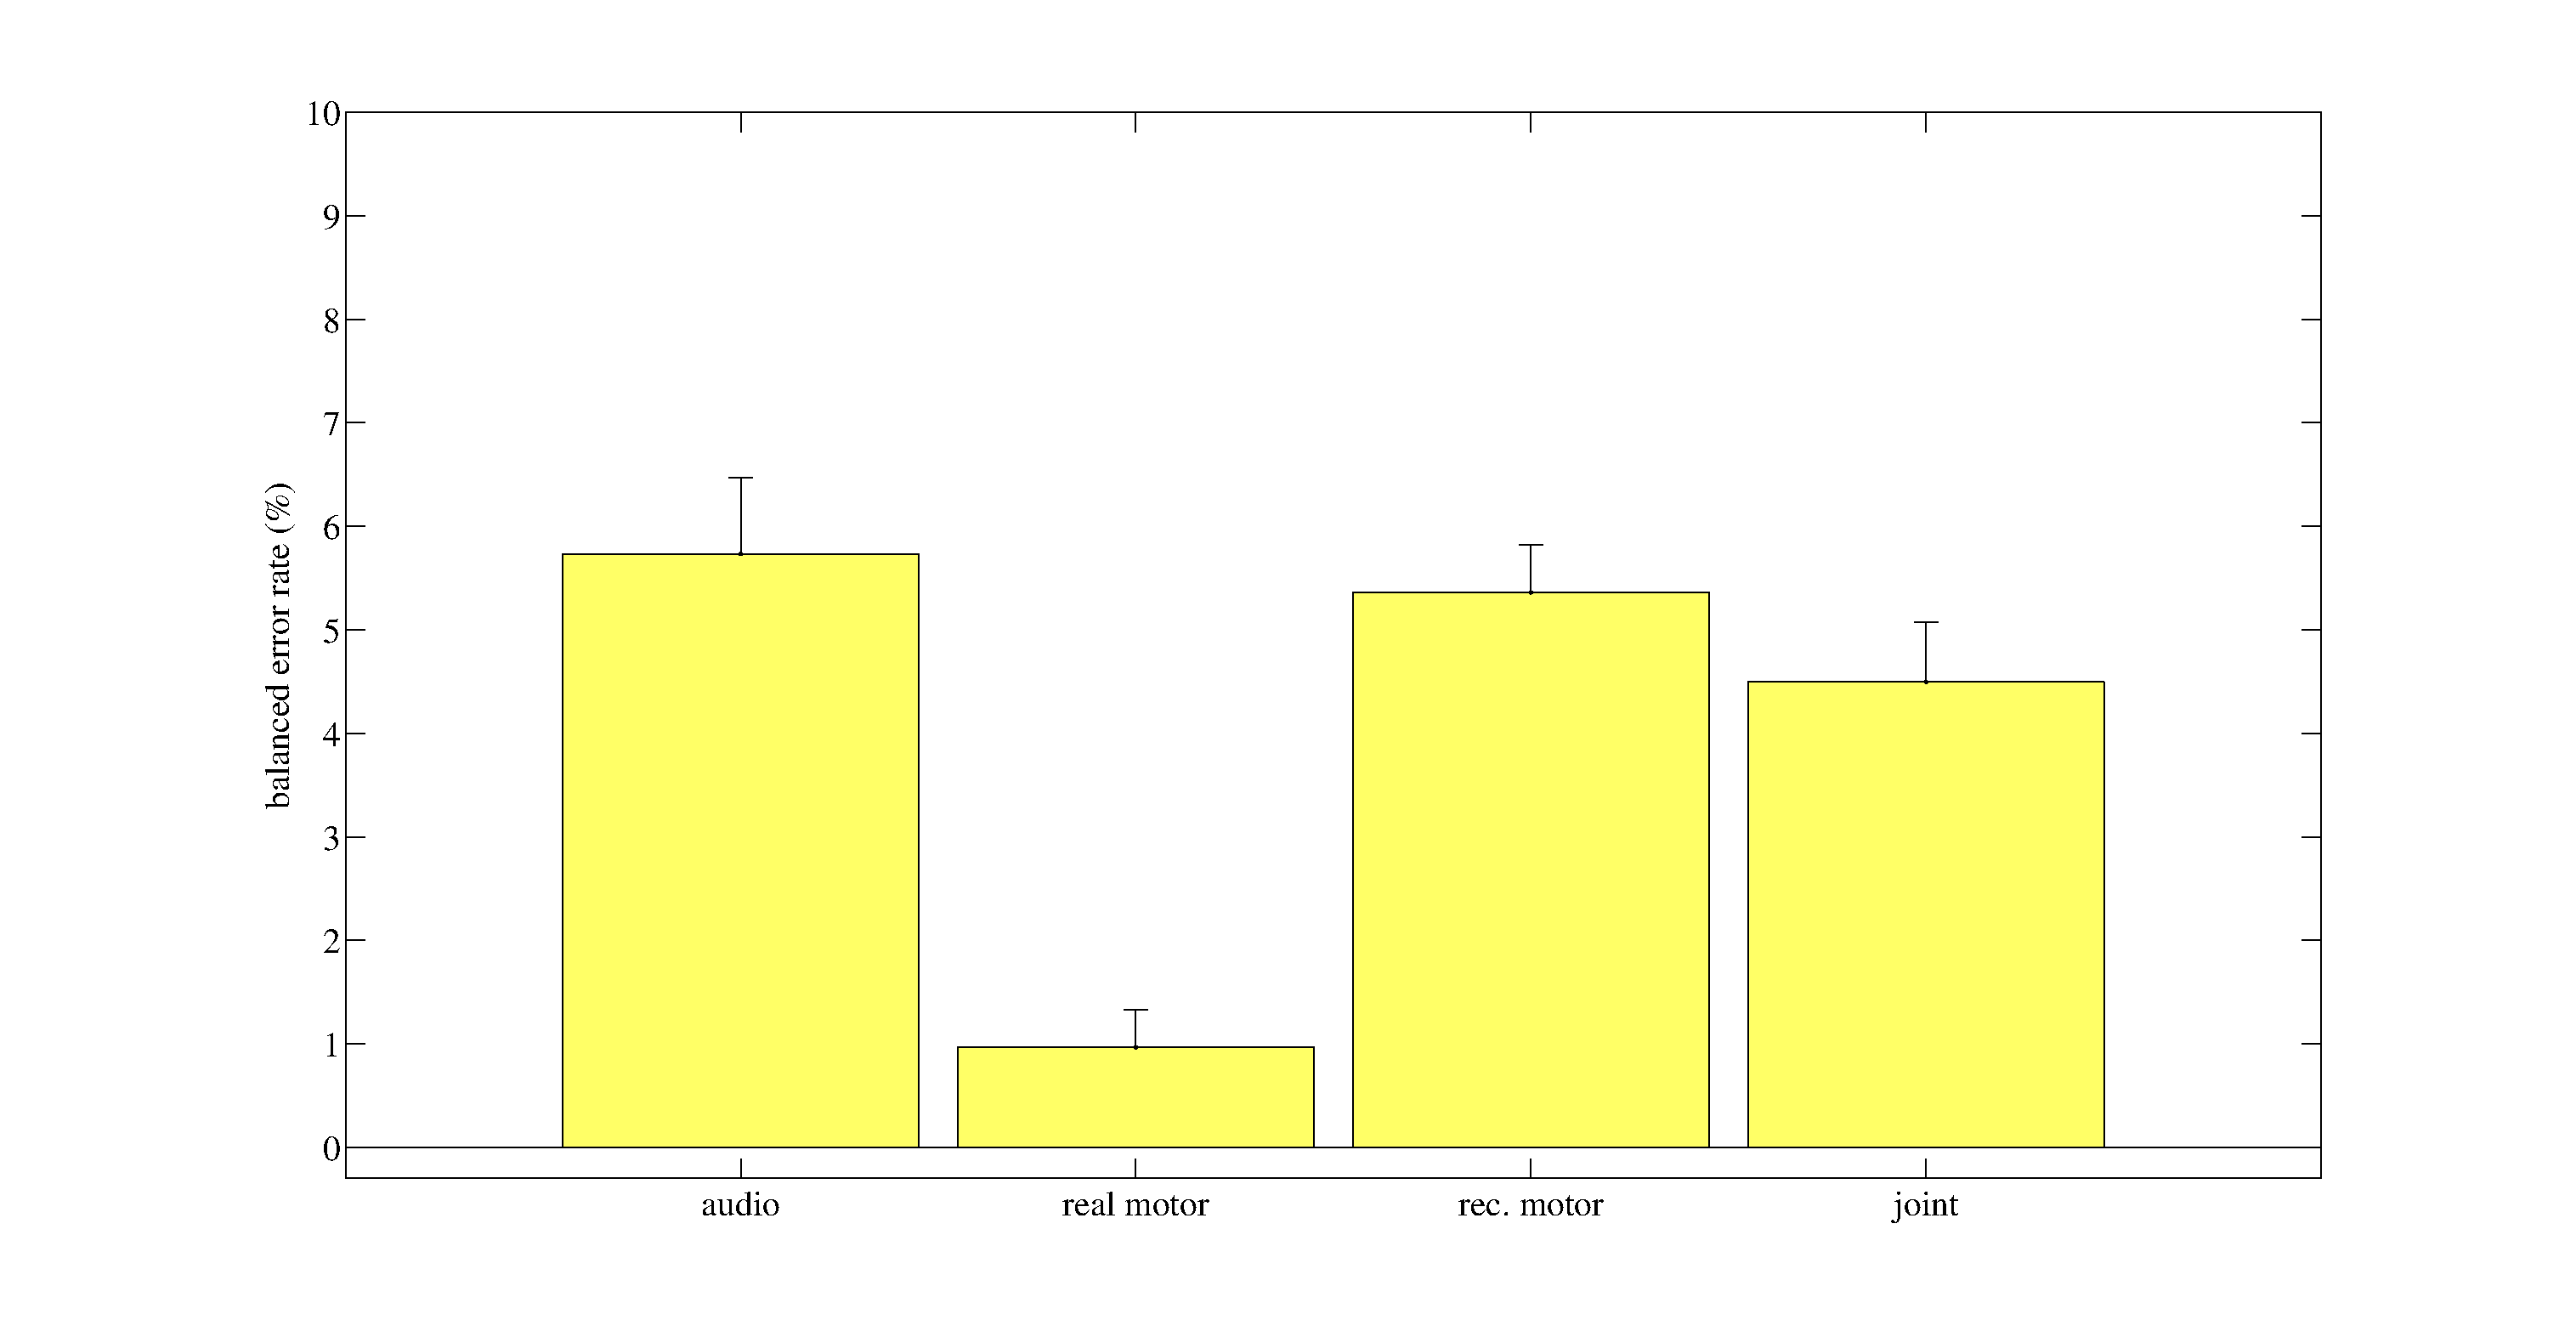
\includegraphics[width=0.45\textwidth]{figs/exp1} &
    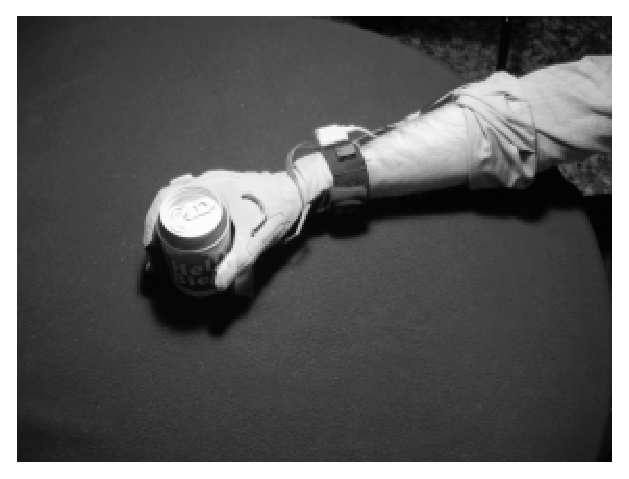
\includegraphics[width=0.45\textwidth]{figs/exp2} \\
    $(a)$ & $(b)$ \\
  \end{tabular}
  \caption{Classification $(a)$ and regression $(b)$ performance
    difference obtained by our method with respect to \emph{NoAdapt}.}
  \label{fig:diff_res}
\end{figure*}

To assess the performance of the proposed adaptation method we
compared it to two baseline methods. The first one, that we call
\emph{Prior}, consists in using only the pre-trained models without
updating them with the new training data. Therefore we consider only the
best performance obtained by one of the $9$ pre-trained models, corresponding to the
best-case scenario. The second one, \emph{NoAdapt}, is plain LS-SVM
using only the new data for training, as it would be in the standard
scenario without adaption.

As a measure of performance, for classification we use the standard
classification rate; for regression, the performance index is the
correlation coefficient evaluated between the predicted force signal
and the real one. The choice of the correlation coefficient, as
opposed to the more standard Mean-Square Error, is suggested by a
practical consideration: when driving a prosthesis, or even a
non-prosthetic mechanical hand, we are not interested in the absolute
force values desired by the user/subject, since mechanical hands
usually cannot apply as much force as human hands do, for obvious
safety reasons\footnote{Or, e.g., in teleoperation scenarios, they
could be able to apply \emph{much more} force than a human hand
can.}. We are rather concerned about getting a signal which is
\emph{strongly correlated} with the user/subject's will.

To build the pre-trained models we used the standard SVM
algorithm. All the parameters to be set during training ($C$ and
$\gamma$ of the gaussian kernel) were chosen by cross-validation. In
the following Figures, error bars (when present) denote $\pm 1$
standard deviations with respect to the average values.

Figure \ref{fig:diff_res} shows the difference in classification
(panel $(a)$) and regression (panel $(b)$) performance obtained by our
method with respect to \emph{NoAdapt}. As one can see, adaptation
uniformly obtains a better performance, with the exception of
classification when the number of samples is below $150$: in that case a
slight loss of about $1\%$ can appear).  In the worst cases, the
performance of \emph{NoAdapt} is re-obtained. Notice also that
standard deviations are rather large when training is done on too few
samples. This is due to the high variance of the leave-one-out error
technique when too few training samples are considered.

Depending on the subject, the improvement can be quite large: up to
about $11\%$ higher rate for classification and $10\%$ stronger
correlation for regression. For classification, the average gain is
almost $5\%$ when there are only $30$ training samples. It settles
to around $1\%$ with smaller standard deviation, as the number of
training samples increases. For regression, it is of about $4\%$
stronger correlation uniformly.

\begin{figure*}[!ht] \centering
  \begin{tabular}{cc}
    \includegraphics[width=0.45\textwidth]{figs/exp1_abs_best} &
    \includegraphics[width=0.45\textwidth]{figs/exp1_abs_worst} \\
    $(a)$ & $(b)$ \\
  \end{tabular}
  \caption{Classification: $(a)$ classification rate gain
    of the adapted model compared to \emph{NoAdapt} and \emph{Prior}
    on the best-case subject; $(b)$ classification rate gain for
    the worst-case subject.}
  \label{fig:cla_abs}
\end{figure*}

\begin{figure*}[!ht] \centering
  \begin{tabular}{cc}
    \includegraphics[width=0.45\textwidth]{figs/exp2_abs_best} &
    \includegraphics[width=0.45\textwidth]{figs/exp2_abs_worst} \\
    $(a)$ & $(b)$ \\
  \end{tabular}
  \caption{Regression: $(a)$ correlation strength gain
    of the adapted model compared to \emph{NoAdapt} and \emph{Prior}
    for the best-case subject; $(b)$ correlation gain for
    the worst-case subject.}
  \label{fig:reg_abs}
\end{figure*}

To get a more detailed idea of the results obtained, consider now Figure \ref{fig:cla_abs},
concerning the classification experiment. Panel $(a)$ shows the
performance obtained on the best-case subject, that is, a subject for
whom a very good match has been found among the pre-trained models,
while panel $(b)$ shows the performance for the worst-case subject. In
the best case the gain is about $3\%$ after 360 samples, while
in the worst case we basically re-obtain the performance of
\emph{NoAdapt}, as soon as enough samples from the new distribution
are considered. Essentially, our method improves things if a good
match can be found, and does no harm if none exists.
Similar observations can be done for the regression task (Figure
\ref{fig:reg_abs}). In the best case, the correlation is about
0.06 points uniformly stronger, whereas in the
worst case \emph{NoAdapt}'s perfomance is obtained.

The worst-case subjects represent the paradigmatic case of no previous
models matching the current distribution; as a consequence, the
parameter $\beta$ was automatically set to a very small value. In this
case, there is essentially no transfer of prior knowledge. But it
is reasonable to claim that the overall performance of the method
would increase along with the number of stored models, since this
would mean a larger probability of finding a matching pre-trained
model.

In the long run, a large database of pre-trained models, possibly
categorised in order to avoid too hard a computational burden, would
definitely help getting uniformly better performances.
